% =============================================================================
% Part 4: Results
% =============================================================================

\section{Results}
\label{sec:results}

The results follow the paper's two movements. The first movement (\S\ref{sec:results_encoding}--\S\ref{sec:results_warmup}) is an anatomy of where in the original SLEEP pipeline information is preserved, transformed, or lost: where encoding succeeds (\S\ref{sec:results_encoding}), why it does not become recall (\S\ref{sec:results_rwr}), what storage granularity is required (\S\ref{sec:results_episodes}), where consolidation stalls (\S\ref{sec:results_consolidation}), what the safety parameters buy (\S\ref{sec:results_pareto}), how the answers change with evaluation horizon (\S\ref{sec:multi_cycle}), and whether the recognition--recall gap yields to a lightweight repair (\S\ref{sec:results_warmup}). The second movement (\S\ref{sec:results_localisation}--\S\ref{sec:results_matrix}) locates the causes of the consolidation failure and validates their removal: a five-arm isolation of substrate and surface diversity (\S\ref{sec:results_localisation}), the discovery that the safety machinery itself was a third cause (\S\ref{sec:results_third_cause}), the repaired pipeline as an autonomous system (\S\ref{sec:results_pipeline_v2}), and the pre-registered four-model validation matrix (\S\ref{sec:results_matrix}).

\subsection{Encoding: LoRA Fast Weights vs. KV Memory Injection}
\label{sec:results_encoding}

\paragraph{Proposed:} The original SLEEP design specified LoRA adapters as the fast-weight substrate. We find this configuration cannot deposit retrievable knowledge from a single inference pass, and we show that direct-write KV memory injection produces a clear---if limited---encoding signal.

\paragraph{Setup:} We compare two $W_{\mathrm{fast}}$ substrates on an identical 200-fact wake-only protocol: (i) LoRA $W_{\mathrm{fast}}$ updated by gradient descent on each tagged span (the original specification), and (ii) KV memory injection with episode storage and top-$k$ retrieval gating ($k=16$). For each, we evaluate multiple-choice accuracy and BCP after wake (no sleep cycle).

\paragraph{Results:} Table~\ref{tab:substrate_comparison} reports the contrast. LoRA $W_{\mathrm{fast}}$ at $\alpha_{\mathrm{fast}} = 10^{-4}$ produces no detectable encoding signal: tagged-fact MC accuracy ($0.23$) is statistically indistinguishable from untagged-fact accuracy ($0.24$). Increasing the learning rate to $10^{-3}$ degrades the model (BCP $1.17$) without producing recall. We attribute this to the bfloat16 precision floor: at $\alpha_{\mathrm{fast}} = 10^{-4}$, single-step gradient updates are below the dtype's representable epsilon for typical weight magnitudes.

\begin{table}[t]
\centering
\caption{$W_{\mathrm{fast}}$ substrate comparison on the 200-fact wake-only protocol. KV injection produces a recognition signal that LoRA does not; KV without retrieval gating destroys BCP.}
\label{tab:substrate_comparison}
\begin{tabular}{lcccc}
\toprule
& MC Tagged & MC Untagged & $\Delta$ (T--U) & BCP \\
\midrule
LoRA $W_{\mathrm{fast}}$ ($\alpha = 10^{-4}$) & 0.23 & 0.24 & $-0.01$ & 0.99 \\
LoRA $W_{\mathrm{fast}}$ ($\alpha = 10^{-3}$) & 0.24 & 0.24 & $0.00$  & 1.17 \\
KV memory (no gating) & 0.27 & 0.16 & $+0.11$ & 96.88 \\
KV memory ($k=16$, gated) & \textbf{0.28} & \textbf{0.12} & $\mathbf{+0.16}$ & \textbf{1.08} \\
\bottomrule
\end{tabular}
\end{table}

KV memory injection with retrieval gating produces a $+0.16$ multiple-choice gap between tagged and untagged facts, with BCP held at $1.08$ (Figure~\ref{fig:substrate}).

\begin{figure}[t]
\centering
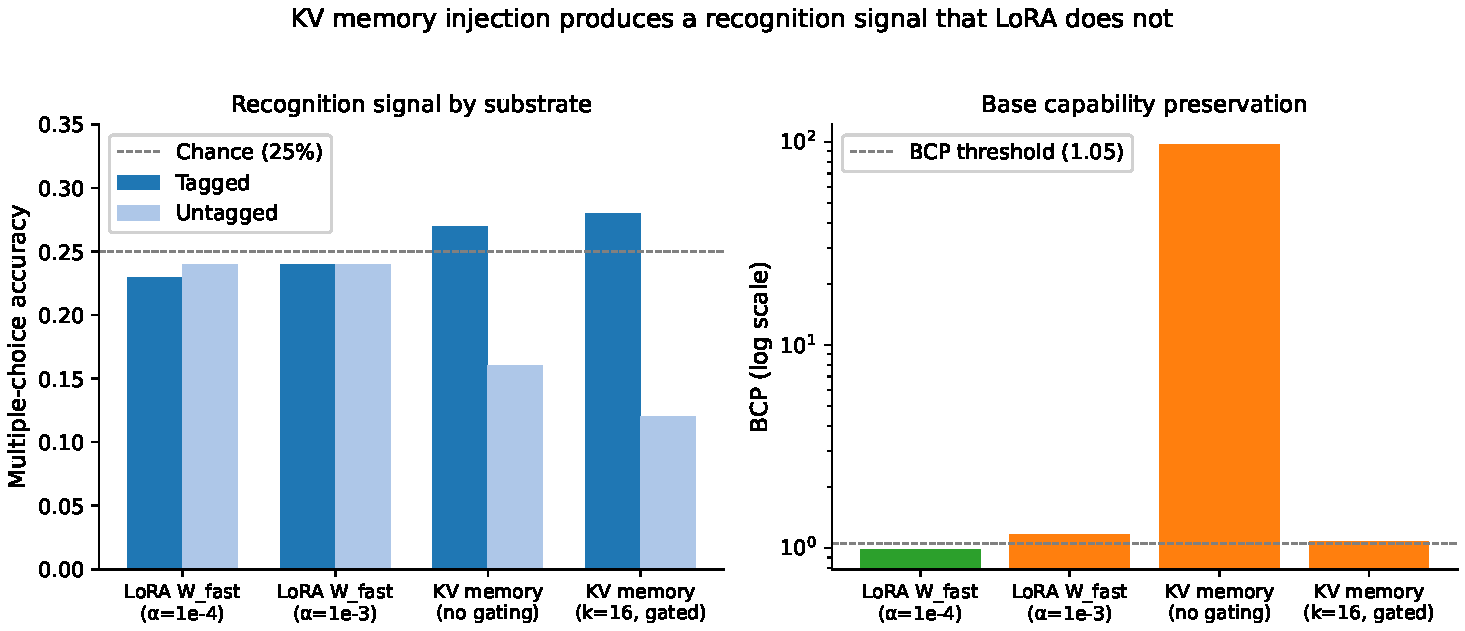
\includegraphics[width=0.95\textwidth]{figures/figure_substrate_comparison.pdf}
\caption{Comparison of $W_{\mathrm{fast}}$ substrates on a 200-fact wake-only protocol. Left: tagged-vs-untagged multiple-choice accuracy. Right: BCP (log scale, since the no-gating KV configuration produces $\sim 100\times$ degradation). The KV substrate with retrieval gating is the only configuration that produces a measurable recognition signal (Tagged $-$ Untagged $= +0.16$) while preserving base capability.}
\label{fig:substrate}
\end{figure}

Calibration analysis is more sensitive: the average probability assigned to the correct option, conditional on the model picking the wrong one, is $0.23$ for tagged facts versus $0.19$ for untagged---suggesting a partial encoding signal that does not quite flip predictions. Without retrieval gating, the KV bank's contents drown attention on irrelevant queries, destroying base capability (BCP $96.88$).

\subsection{Recognition Without Recall}
\label{sec:results_rwr}

The KV memory result above is structurally partial. Tagged-fact \emph{multiple-choice} accuracy exceeds untagged by $+0.16$, but tagged-fact \emph{cloze} accuracy is $0.00$ and tagged-fact \emph{free-form} accuracy is $0.00$. The same memories that bias four-way recognition fail to drive autoregressive token generation. We name this dissociation the \emph{recognition--recall gap} and treat it as the paper's central \emph{diagnostic} finding: it is not a defect of our specific implementation but, we argue, a structural property of memory-augmented attention over frozen pretrained models. It concerns the KV-injection path specifically and stands independently of the consolidation repair reported in the second movement---the repair routes knowledge into weights, not through injected attention, and the gap for injected memory remains.

\paragraph{The cognitive-psychology analogue:} The recognition--recall dissociation is a foundational observation in episodic memory research \citep{morris2006elements}. Recognition (``does this seem familiar?'') can be supported by partial trace reactivation---a sense of fluency or matching---while free recall (``what came next?'') requires reconstructing the trace in sufficient completeness to generate its content. Patients with hippocampal damage often retain residual recognition ability even when free recall is severely impaired. The structural distinction in cognitive psychology is that recognition is a similarity-judgment task (compare the probe to stored representations), while recall is a generation task (produce the stored representation autoregressively from a cue). Our result reproduces this distinction in transformer language models for a different reason at the mechanistic level, but with the same operational consequence.

\paragraph{The mechanistic explanation:} At each generation step, attention to memory K/V provides additive perturbations to the pre-softmax logits at every layer. For our $n_{\mathrm{mem}} \approx 5{,}500$ stored tokens with top-$k$ retrieval gating, the $k$ retained memory positions contribute at most $k/(k + |\text{seq}|)$ of total attention mass, with the remainder going to the current sequence's tokens whose keys are RoPE-anchored at the model's normal training distribution. Memory thus enters the next-token prediction as a small perturbation against a strong prior trained on trillions of tokens. The perturbation is sufficient to flip an argmax in a four-way comparison---all four options share the same prior and the memory tilts the relative scores---but is overwhelmed across an autoregressive generation, where each generated token comes from a categorical distribution over a 150{,}000-token vocabulary in which the prior dominates. A memory entry can nudge the most likely token of a sentence; it cannot consistently steer 50 generated tokens against the model's natural continuation distribution.

\paragraph{Why this matters beyond SLEEP:} Memorizing Transformers, of Wu et al., avoid exactly this failure mode by retraining the model on memory-augmented losses, teaching the next-token distribution to depend on retrieved K/V \citep{wu2022memorizing}. Our recognition-without-recall result is---in part---a precise specification of \emph{what} that fine-tuning fixes: the gap between attention-time bias and sampling-time use. For applications that need a frozen pretrained backbone with appended memory, the gap is structural and cannot be closed by hyperparameter tuning. We return to the architectural implications in Section~\ref{sec:discussion}.

\subsection{Episode Storage: Tags Are Pointers}
\label{sec:results_episodes}

\paragraph{Proposed:} The original formalization stored only tagged-token K/V; we show this captures entity mentions without their factual content, and that storing the full sentence containing the tag is necessary for replay quality.

\paragraph{Diagnostic:} We inspect the generated replays produced by the sleep cycle when the bank stores only the tagged span. With seeds like ``\texttt{Nimbus Holdings reported Q}'', the model generates fluent financial-news text with fabricated revenue figures (``\texttt{\$32.6 million}'', ``\texttt{up 6.1\% from prior year}'')---values not in the original fact. The pattern persists across templates: stored entity-name K/V provide an attention bias toward ``earnings statement'' representations without supplying the specific facts.

When storage is expanded to the full sentence containing the tag (the \emph{episode}), and the seed for replay generation is taken from the start of the episode rather than from the tag location, replay coherence improves: the consolidation rate (validation passes / candidates) rises from $40\%$ to $62\%$, and BCP improves from $1.06$ to $1.008$ ($k=16$, episode storage). The recall metrics, however, do not improve correspondingly---a finding we examine in Section~\ref{sec:results_consolidation}.

This empirical correction validates the proposal's own framing: \emph{tags are pointers, not storage}. The implementation must store what the pointer indexes, not the pointer's surface form.

\subsection{The Consolidation Bottleneck}
\label{sec:results_consolidation}

\paragraph{Proposed:} Even when generative replay is replaced with the original tokens (eliminating replay-quality as a confound), SLEEP's safety machinery prevents sufficient $W_{\mathrm{cons}}$ updates for free-form recall.

\paragraph{Setup:} We add a \emph{replay-strategy} parameter to the sleep engine. With \texttt{replay\_strategy="original"}, the engine bypasses generation entirely and uses the original fact tokens as replays. All other components---PRP allocation, EWC, hard clipping, validation, rollback, KV-disabled training---run unchanged. This isolates ``does $W_{\mathrm{cons}}$ training learn from data, given perfect data?''

\paragraph{Result:} With original-token replays under default safety parameters ($\delta_{\max}=0.01$, $\lambda_{\mathrm{EWC}}=100$, $\alpha_{\mathrm{slow}}=10^{-4}$, $\sim$100 steps), recall remains at floor across five seeds: $\mathrm{DRA} = 0.006 \pm 0.003$ with $\mathrm{BCP} = 1.066 \pm 0.032$. Perfect replay data does not rescue consolidation.

\paragraph{Quantifying the self-grading discrepancy:} To measure---rather than argue---the mismatch between internal and external criteria, we add a second validation stage. Stage one is the original surprise-reduction check; stage two is a direct free-form recall test that asks whether the post-training model can produce any expected keyword from the fact's question prompt under greedy decoding. Table~\ref{tab:two_stage} reports both gates across five seeds.

\begin{table}[t]
\centering
\caption{Two-stage validation across five seeds (200 facts, original-token replay). The surprise proxy confirms roughly 39 consolidations per run; fewer than one survives a direct recall test.}
\label{tab:two_stage}
\begin{tabular}{lcc}
\toprule
Quantity & Mean $\pm$ SD & Per-seed values \\
\midrule
Passed surprise-reduction (stage 1) & $38.8 \pm 0.4$ & 39, 39, 39, 39, 38 \\
Passed direct recall gate (stage 2) & $0.4 \pm 0.5$ & 0, 1, 1, 0, 0 \\
$\mathrm{DRA}$ & $0.006 \pm 0.003$ & .005, .007, .010, .003, .005 \\
$\mathrm{BCP}$ & $1.066 \pm 0.032$ & 1.11, 1.03, 1.04, 1.09, 1.06 \\
\bottomrule
\end{tabular}
\end{table}

The gap is a factor of roughly one hundred: \textbf{$\sim$97\% of the consolidations the system certifies internally fail an external recall test}, and the effect is consistent on every seed. \emph{Internal validation criteria can pass while external recall fails.} We argue this self-grading discrepancy is a methodological concern broader than SLEEP: a system that grades itself on a proxy of its own behavior provides no protection against proxy--target mismatch, and the magnitude here suggests the mismatch can be near-total rather than marginal.

\paragraph{Cross-family and cross-scale replication:} Because both the recall floor and the self-grading gap could in principle be artefacts of one model's pretraining, we repeat the five-seed protocol on three further models spanning two additional configurations of the same family and two other families. Table~\ref{tab:cross_model} shows the outcome: the free-form recall floor sits at $\mathrm{DRA} \approx 0.006$--$0.007$ on every model, and the direct recall gate confirms at most a fraction of one consolidation per run everywhere, against 4--39 proxy confirmations. The number of \emph{candidates} varies substantially across families---Mistral's surprise statistics allocate a tenth as many as Qwen---but the false-confirmation structure is invariant. Notably, the same models follow in-context facts well (Table~\ref{tab:baselines}), so the parametric recall floor is not a comprehension failure.

\begin{table}[t]
\centering
\caption{The recall floor and self-grading gap across four models, three families (5 seeds each, mean $\pm$ SD). The floor and the proxy--recall mismatch replicate everywhere.}
\label{tab:cross_model}
\begin{tabular}{lcccc}
\toprule
Model & DRA & BCP & Proxy passes & Recall-gate passes \\
\midrule
Qwen2.5-7B    & $0.006 \pm 0.003$ & $1.066 \pm 0.032$ & $38.8 \pm 0.4$ & $0.4 \pm 0.5$ \\
Qwen2.5-1.5B  & $0.007 \pm 0.002$ & $0.997 \pm 0.003$ & $23.8 \pm 1.1$ & $0.0 \pm 0.0$ \\
Llama-3.1-8B  & $0.006 \pm 0.003$ & $0.958 \pm 0.009$ & $9.2 \pm 2.4$  & $0.6 \pm 0.5$ \\
Mistral-7B    & $0.007 \pm 0.000$ & $1.001 \pm 0.002$ & $4.0 \pm 1.0$  & $0.0 \pm 0.0$ \\
\bottomrule
\end{tabular}
\end{table}

\subsection{The Stability--Plasticity Pareto Frontier}
\label{sec:results_pareto}

\paragraph{Proposed:} Sweeping the four safety knobs produces a smooth Pareto curve with no operating point achieving both meaningful recall and preservation on the single-cycle benchmark.

\paragraph{Setup:} Using original-token replay (clean signal), we sweep four settings of $(\delta_{\max}, \lambda_{\mathrm{EWC}}, \alpha_{\mathrm{slow}}, \mathrm{steps\_per\_memory})$ from SLEEP defaults to near-naive-LoRA. We compare against naive LoRA fine-tuning at matched compute. Table~\ref{tab:pareto} reports the curve; Figure~\ref{fig:pareto} plots it.

\begin{figure}[t]
\centering
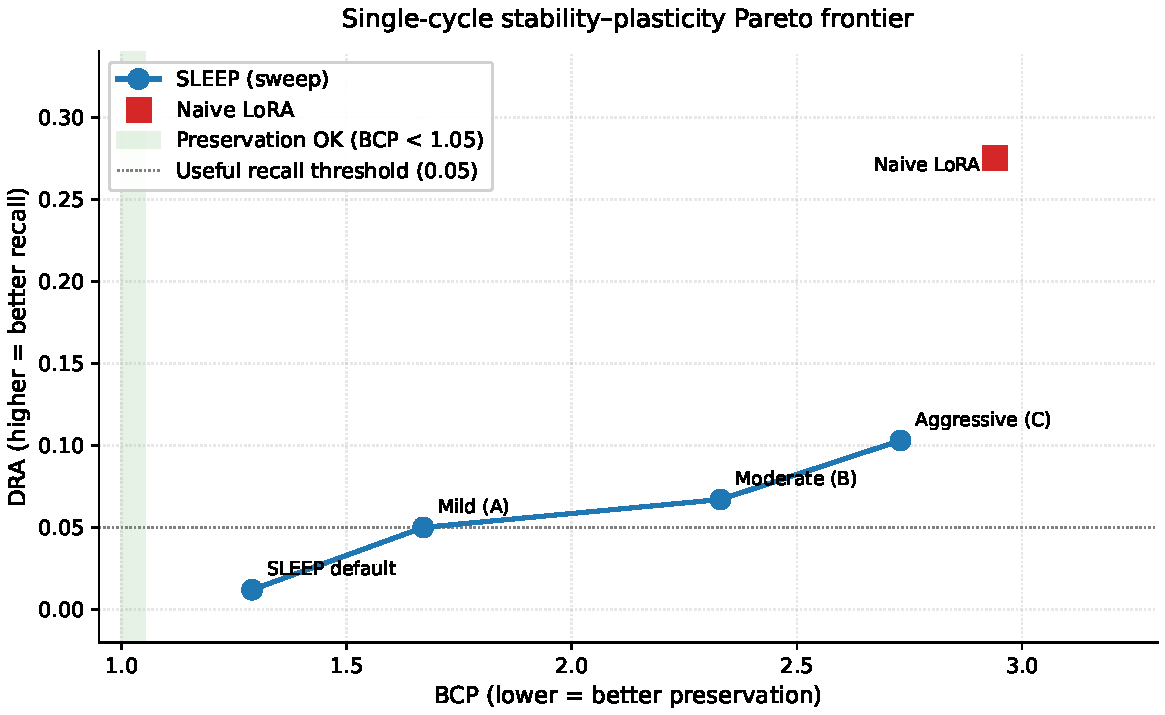
\includegraphics[width=0.78\textwidth]{figures/figure_pareto_frontier.pdf}
\caption{Single-cycle stability--plasticity Pareto frontier of the \emph{original} architecture (attention-top placement, single-wording replay). The green band shows the preservation-acceptable region ($\mathrm{BCP} < 1.05$); the dotted line shows a useful-recall threshold ($\mathrm{DRA} > 0.05$). No setting on this frontier reaches the upper-left intersection---and Section~\ref{sec:results_localisation} shows why: the frontier itself is an artefact of consolidating into the wrong substrate. The repaired pipeline of Section~\ref{sec:results_pipeline_v2} reaches $\mathrm{DRA}=0.189$ at $\mathrm{BCP}=0.88$ on this model (five seeds), inside the region this curve suggested was unreachable.}
\label{fig:pareto}
\end{figure}

\begin{table}[t]
\centering
\caption{Single-cycle Pareto frontier on the 200-fact benchmark. No SLEEP setting achieves $\mathrm{DRA} > 0.05$ with $\mathrm{BCP} < 1.05$. Naive LoRA achieves higher DRA at unacceptable BCP cost.}
\label{tab:pareto}
\begin{tabular}{lcccccc}
\toprule
Setting & $\delta_{\max}$ & $\lambda_{\mathrm{EWC}}$ & $\alpha_{\mathrm{slow}}$ & steps/mem & DRA & BCP \\
\midrule
SLEEP default     & 0.01     & 100  & $10^{-4}$ & 5  & 0.012 & 1.29 \\
Mild relax (A)    & 0.02     & 50   & $10^{-4}$ & 4  & 0.050 & 1.67 \\
Moderate (B)      & 0.05     & 10   & $3{\times}10^{-4}$ & 4  & 0.067 & 2.33 \\
Aggressive (C)    & 0.10     & 1    & $5{\times}10^{-4}$ & 6  & 0.103 & 2.73 \\
Naive LoRA        & $\infty$ & 0    & $10^{-4}$ & --- & 0.275 & 2.94 \\
\bottomrule
\end{tabular}
\end{table}

The curve (Figure~\ref{fig:pareto}) is monotonic: relaxing safety raises DRA and raises BCP simultaneously. There is no knee; no inflection point where DRA jumps without BCP cost. On a single-cycle 200-fact benchmark, the original architecture's value proposition---``a small recall sacrifice in exchange for guaranteed preservation''---does not hold: every SLEEP point pays more BCP per percentage point of recall than naive LoRA does at its single endpoint. Within this movement of the paper the frontier reads as a stability--plasticity wall; Section~\ref{sec:results_localisation} will show it is better read as the cost curve of writing to the wrong substrate.

\paragraph{Reference points:} Table~\ref{tab:baselines} places these numbers against three baselines that bound the problem. Supplying the fact in context yields $\mathrm{DRA} = 0.760$ at no preservation cost, establishing that the model reads and uses a fact it can see; RAG's shortfall against that ceiling ($0.213$) is therefore attributable to retrieval rather than to comprehension. Most pointedly, EWC applied alone---without hard clipping, interleaving, validation rollback, tagging, or sleep scheduling---reaches $\mathrm{DRA} = 0.070$ at $\mathrm{BCP} = 1.116$, a better recall-per-preservation ratio than any full SLEEP configuration in Table~\ref{tab:pareto}.

\begin{table}[t]
\centering
\caption{Baseline reference points across models (100 facts, single seed each). In-context injection bounds the task from above everywhere; on 7B-class models EWC-only achieves a better recall-per-preservation ratio than any full SLEEP configuration, though the effect weakens at 1.5B.}
\label{tab:baselines}
\begin{tabular}{lcccc}
\toprule
& Qwen-7B & Qwen-1.5B & Llama-8B & Mistral-7B \\
\midrule
In-context DRA & 0.760 & 0.700 & 0.987 & 0.927 \\
RAG DRA        & 0.213 & 0.460 & 0.520 & 0.563 \\
EWC-only DRA (BCP) & 0.070 (1.12) & 0.033 (1.43) & 0.073 (1.47) & 0.157 (2.53) \\
\bottomrule
\end{tabular}
\end{table}

\paragraph{Single-cycle interpretation:} A natural reading of these single-cycle results is that SLEEP's safety machinery is over-engineered. The mechanisms (EWC, hard clipping, interleaving, validation rollback) collectively dampen learning more than they protect base capability, and the EWC-only baseline suggests that the marginal machinery beyond the Fisher penalty is not paying for itself. On a one-shot benchmark, that is a true description of what they do. Section~\ref{sec:multi_cycle} tests whether it remains true as the horizon lengthens.

\subsection{Evaluation Horizon and Seed: The Long-Run Comparison Is Not Stable}
\label{sec:multi_cycle}

\paragraph{Proposed:} SLEEP's safety mechanisms are designed for repeated-cycle continual learning rather than single-cycle benchmarks. We therefore evaluate in that regime---and find that the comparison against naive fine-tuning is not stable in the number of cycles, which changes what can be claimed.

\paragraph{Setup:} We split 200 facts into 10 disjoint batches of 20. Across ten sequential cycles the model sees one batch per cycle. After each cycle we measure (i) DRA on the cumulative facts seen so far (the forgetting test), (ii) DRA on the current cycle's facts (the learning test), and (iii) BCP on controls (the preservation test). We compare \textbf{SLEEP-A} (Setting A from the Pareto sweep) against \textbf{Naive LoRA} (200 steps per cycle on that cycle's batch). Both arms accumulate weight updates across cycles---each cycle starts from the previous cycle's adapter state. We run this protocol with three seeds on Qwen2.5-7B and two seeds on each of Qwen2.5-1.5B, Llama-3.1-8B, and Mistral-7B: nine SLEEP runs and nine naive runs in total.

\begin{table}[t]
\centering
\caption{Ten-cycle continual learning across four models (cycle-10 endpoints). ``Plateau from'' gives the cycle at which the SLEEP arm's BCP stops changing. Every SLEEP run shows a step-then-plateau trajectory; the plateau \emph{level} varies by orders of magnitude across seeds of the same configuration.}
\label{tab:multi_cycle}
\begin{tabular}{llcccc}
\toprule
Model & Seed & SLEEP BCP@10 (plateau from) & Naive BCP@10 & SLEEP DRA & Naive DRA \\
\midrule
Qwen-7B   & 0 & 4.53 (c4)   & 3.36 & 0.050 & 0.085 \\
Qwen-7B   & 1 & 10.20 (c3)  & 6.42 & 0.032 & 0.080 \\
Qwen-7B   & 2 & 2.71 (c5)   & 5.44 & 0.057 & 0.078 \\
Qwen-1.5B & 0 & 15.96 (c3)  & 21.01 & 0.045 & 0.035 \\
Qwen-1.5B & 1 & 230.1 (c5)  & 45.83 & 0.012 & 0.048 \\
Llama-8B  & 0 & 4.83 (c3)   & 6.09 & 0.032 & 0.083 \\
Llama-8B  & 1 & 1530.9 (c3) & 7.11 & 0.045 & 0.075 \\
Mistral-7B & 0 & 3.22 (c2)  & 2.90 & 0.008 & 0.192 \\
Mistral-7B & 1 & 1.64 (c2)  & 3.72 & 0.003 & 0.160 \\
\bottomrule
\end{tabular}
\end{table}

\begin{figure}[t]
\centering
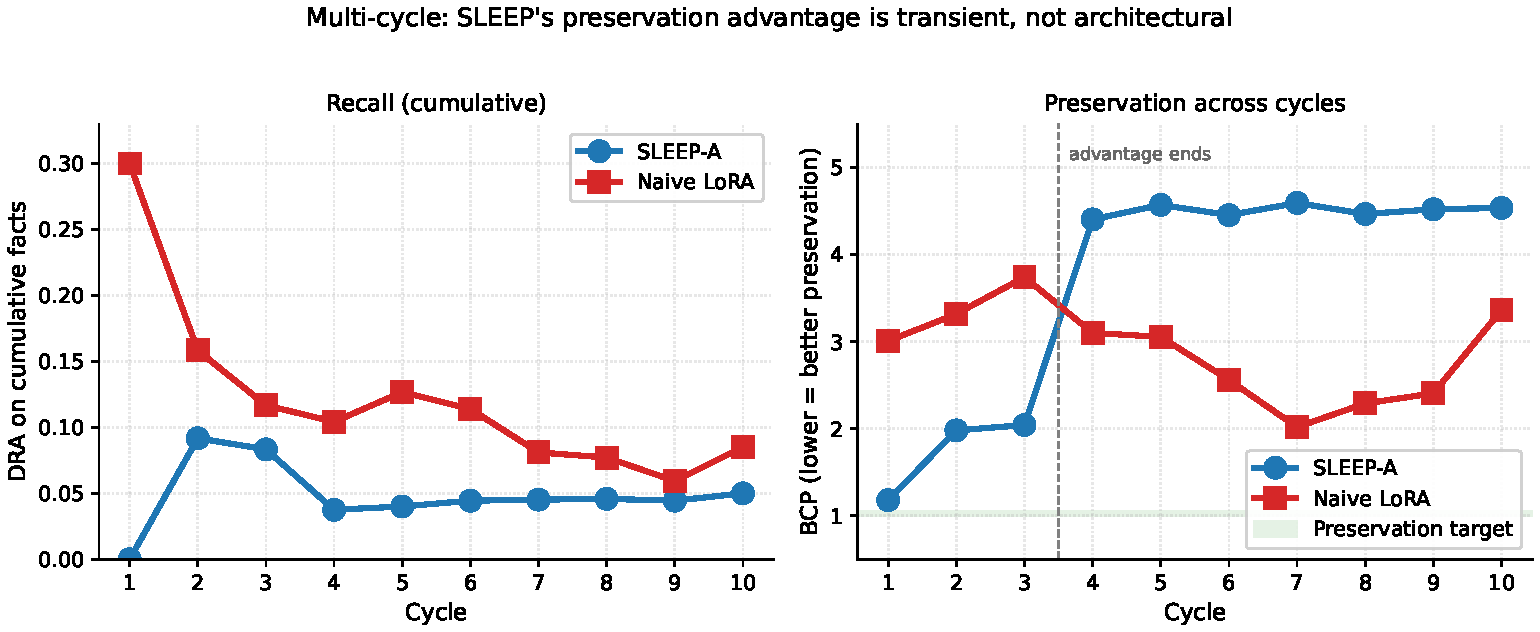
\includegraphics[width=0.95\textwidth]{figures/figure_multi_cycle.pdf}
\caption{Ten-cycle continual learning on disjoint batches (Qwen2.5-7B, seed 0 shown; Table~\ref{tab:multi_cycle} reports all nine run-pairs). Left: cumulative DRA. Right: BCP with the crossover marked. SLEEP's preservation advantage holds for three cycles, after which its BCP steps to a plateau while naive LoRA fluctuates.}
\label{fig:multi_cycle}
\end{figure}

\paragraph{Result---a universal shape with a lottery for its level:} Table~\ref{tab:multi_cycle} reports all nine run-pairs. Three regularities hold in every run. First, the \emph{step-then-plateau} signature: each SLEEP run holds BCP near 1 for its first cycles, then jumps discretely and stays flat---within a few percent---for every remaining cycle (9/9 runs). Second, naive LoRA's cumulative recall exceeds SLEEP's in 8 of 9 pairs, typically by $2$--$20\times$. Third, no run of either arm ever satisfies $\mathrm{BCP} < 1.05$ beyond cycle two. What does \emph{not} replicate is the plateau level: across seeds of the \emph{same configuration} it spans $2.7$--$10.2$ on Qwen-7B, $16$--$230$ on Qwen-1.5B, and $4.8$--$1531$ on Llama---three orders of magnitude on identical hyperparameters. Which arm ``wins'' preservation at cycle 10 accordingly flips seed to seed (SLEEP wins 4 of 9 pairs, naive 5 of 9).

\paragraph{Interpretation---horizon and variance jointly decide the ordering:} Three successively larger experiments gave three different headlines: a single cycle favours naive LoRA; three cycles favour SLEEP (the ordering we ourselves reported from the three-cycle experiment); ten cycles across seeds shows the ordering is not stable at all. The seed-stable claims are structural, not comparative: SLEEP's clipping mechanism caps damage at a plateau whose \emph{existence} is guaranteed but whose \emph{level} is effectively a lottery over the optimisation path---consistent with $\delta_{\max}$ saturation geometry, where the clip freezes whatever damage has accumulated when saturation is reached---and the unconstrained baseline buys its consistently higher recall with wildly fluctuating damage. We conclude that \textbf{single-run, fixed-horizon comparisons of continual-learning architectures are unreliable at both of the scales this field typically reports}, and recommend that such comparisons state a horizon sweep and a seed spread or not be made.

\paragraph{What this result does \emph{not} show:} It does not show SLEEP's safety machinery is useless---in 4 of 9 pairs it produced the better cycle-10 preservation, and its early-cycle protection is real everywhere. It shows the machinery does not deliver a \emph{reliable} advantage, and that the aspirational target---BCP near 1 across many cycles while DRA accumulates---was met by no run of either arm. Section~\ref{sec:results_matrix} revisits this protocol with the repaired pipeline and finds that the seed lottery was a property of the \emph{choked} configuration: once consolidation writes to the correct substrate under a moderate clip, the constrained arm's trajectories become smooth and seed-stable, while the lottery persists in---and at small scale destroys---the unconstrained baseline.

\subsection{Repairing the Gap: A Retrieval-Aware Warm-Up}
\label{sec:results_warmup}

\paragraph{Proposed:} The recognition--recall diagnosis of Section~\ref{sec:results_rwr} implies a specific repair: teach the frozen model to use KV memory during generation before asking it to consolidate. If the gap is a missing \emph{skill} rather than a structural limit, a lightweight warm-up should narrow it.

\paragraph{Setup:} We run the warm-up of Section~\ref{sec:warmup_method} on 400 WikiText-2 passages disjoint from the evaluation facts, then re-run the identical recognition and recall evaluation on the 200-fact benchmark with the trained component frozen. We test two capacities: the \emph{gate only} ($36$ parameters) and \emph{gate + LoRA}, in which $W_{\mathrm{cons}}$ trains alongside. Success was pre-registered as $\mathrm{DRA} \in [0.10, 0.15]$ at $\mathrm{BCP} < 1.5$.

\begin{table}[t]
\centering
\caption{Retrieval-aware warm-up across four models (two seeds per variant per model; $\Delta$DRA ranges span seeds). Recall moves by at most $\pm 0.008$ anywhere. The gate-only variant is harmless but inert; the $+$LoRA variant learns its objective yet damages base capability by a family-dependent, sometimes catastrophic amount.}
\label{tab:warmup}
\begin{tabular}{llcc}
\toprule
Model & Variant & $\Delta$DRA (seeds) & BCP after (seeds) \\
\midrule
Qwen-7B    & gate only & $+0.002, +0.002$ & $\sim$1.00, $\sim$1.00 \\
Qwen-7B    & $+$ LoRA  & $+0.003, +0.000$ & 1.73, 3.74 \\
Qwen-1.5B  & gate only & $+0.002, -0.002$ & 1.13, 1.13 \\
Qwen-1.5B  & $+$ LoRA  & $+0.002, -0.002$ & 5.83, 19.9 \\
Llama-8B   & gate only & $-0.007, +0.002$ & 1.78, 1.79 \\
Llama-8B   & $+$ LoRA  & $-0.008, -0.002$ & $1.5{\times}10^{5}$, $1.5{\times}10^{6}$ \\
Mistral-7B & gate only & $+0.008, -0.002$ & 2.77, 3.03 \\
Mistral-7B & $+$ LoRA  & $-0.002, -0.005$ & $1.8{\times}10^{4}$, $1.0{\times}10^{5}$ \\
\bottomrule
\end{tabular}
\end{table}

\begin{figure}[t]
\centering
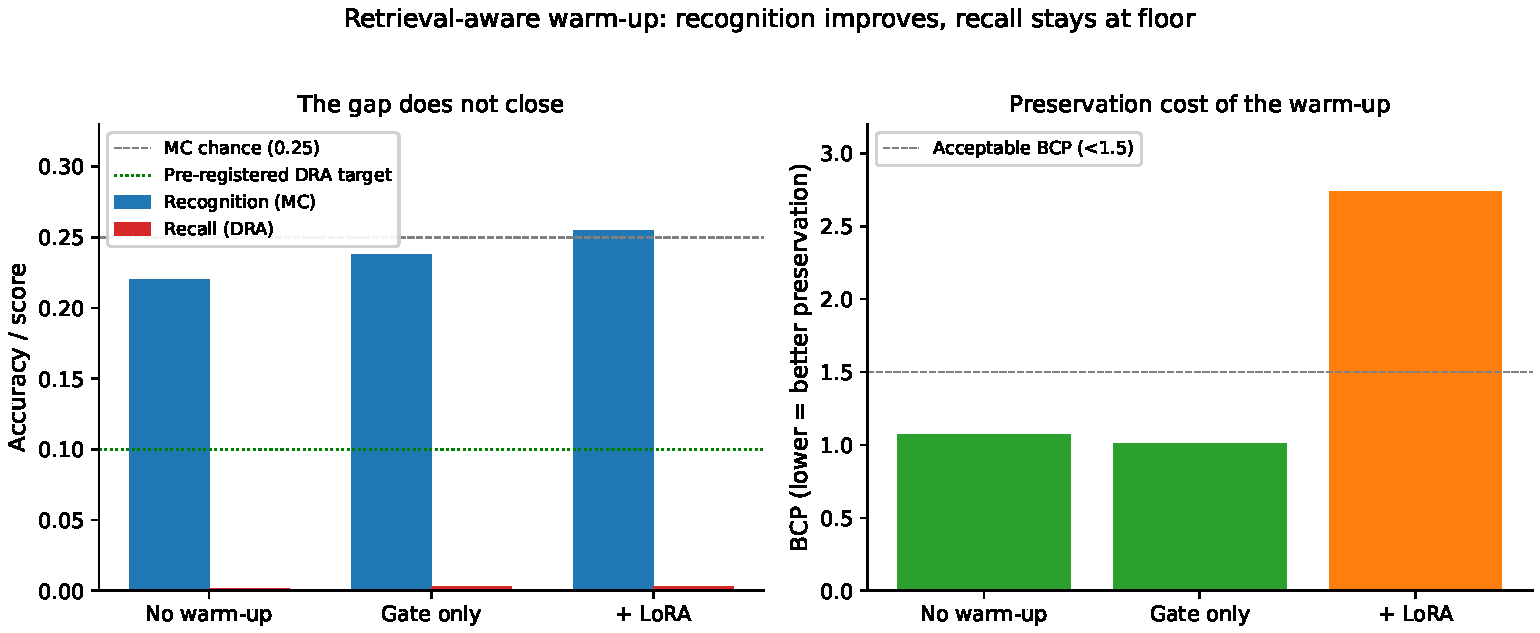
\includegraphics[width=0.95\textwidth]{figures/figure_warmup_extension.pdf}
\caption{Warm-up extension results. Left: recognition (MC) and recall (DRA) under each condition; the pre-registered DRA target is marked. Recognition rises above chance while recall stays at floor. Right: the preservation cost, showing that the higher-capacity variant buys its small recognition gain with substantial base-capability degradation.}
\label{fig:warmup}
\end{figure}

\paragraph{Result---two distinct failure modes, replicated across families:} The gate-only variant does not train: its loss is flat and the learned scales converge to $0.99$--$1.00$, i.e.\ the optimizer finds that the identity is locally optimal. Thirty-six parameters modulating a memory signal cannot manufacture the capability to use it. The gate + LoRA variant \emph{does} learn the objective---on every model the warm-up loss falls substantially (e.g.\ $4.30 \to 3.33$ on Qwen-7B), confirming genuine acquisition of memory-conditioned prediction---and recognition improves modestly where the model survives (MC $0.220 \to 0.270$ on Qwen-7B, seed 0). But recall does not follow anywhere: across sixteen warm-up runs on four models, $|\Delta\mathrm{DRA}| \leq 0.008$ (Table~\ref{tab:warmup}). Meanwhile the LoRA variant's preservation cost is family-dependent and sometimes catastrophic: mild on Qwen-7B (BCP 1.7--3.7), severe on Qwen-1.5B (5.8--19.9), and destructive on Llama and Mistral (BCP $10^{4}$--$10^{6}$) at the same untuned learning rate. Two further observations: when LoRA is present the gate remains pinned at exactly $1.000$ (gradient flows to the higher-capacity component), and on Mistral the gate-only warm-up substantially \emph{reduced} the interference cost of carrying a populated memory bank (BCP with bank active: $8.9 \to 2.8$)---the gate learns to damp memory it cannot learn to exploit.

\paragraph{Interpretation:} The honest statement carries its scope. \textbf{A lightweight retrieval-aware warm-up---$\leq$300 steps on a general corpus, with either a minimal gate or a rank-16 adapter---does not close the recognition--recall gap on any of four models spanning three families.} What it does do is deepen the original diagnosis in two ways. First, the gap survived a principled intervention drawn from published precedent \citep{wu2022memorizing,gmemllm2026,wang2024memoryllm}, replicated across families---stronger evidence of its structural character than any single-model observation. Second, the intervention moved recognition and recall \emph{differentially}---the same training that raised MC accuracy left free-form generation untouched---which is precisely the dissociation the paper names, now reproduced under an experimental manipulation rather than merely observed. We note the caveat that the warm-up learning rate was not tuned per family, which the Llama and Mistral collapses underline; a per-family-tuned variant is cheap follow-up work. We do not claim that retrieval-aware training cannot close the gap; Memorizing Transformers demonstrates that full-scale memory-augmented pretraining does. We claim that the cheap version does not, and we report the scale at which we tested it.

This closes the first movement. Every route into the failure so far---perfect replay data, relaxed safety sweeps, a trained retrieval skill---treated the consolidation target as given. The sections that follow question the target itself.

\subsection{Localising the Failure: Substrate and Surface Diversity}
\label{sec:results_localisation}

\paragraph{Hypothesis:} The knowledge-editing literature (Section~\ref{sec:related}) predicts that factual associations live in mid-stack MLP modules, not the top-third attention projections where biological analogy placed $W_{\mathrm{cons}}$---and that single-wording training should produce string memorization rather than extractable knowledge. If correct, the recall floor of Section~\ref{sec:results_consolidation} is a localisation error, not a stability--plasticity limit.

\paragraph{Setup:} Five arms isolate the two factors on 50 facts at matched exposure (1{,}200 training steps), on Qwen2.5-7B and Llama-3.1-8B, two seeds, safety clipping disabled so that placement and data are the only variables. Arms: (i) attention-top placement, single wording (the original); (ii) mid-MLP placement, single wording; (iii) mid-MLP with paraphrase diversity; (iv) context distillation into mid-MLP with paraphrases; (v) context distillation into attention-top (the placement control for the objective). Evaluation is greedy throughout.

\begin{table}[t]
\centering
\caption{Five-arm localisation ladder (50 facts, matched exposure, clipping disabled; Qwen2.5-7B shown, seed means). Placement, diversity, and objective stack. Cloze and free-form move in \emph{opposite} directions when paraphrases are introduced: the model stops memorizing the string and starts knowing the fact.}
\label{tab:ladder}
\begin{tabular}{lccc}
\toprule
Arm & Free-form DRA & Cloze & BCP \\
\midrule
attention-top, single wording (original) & 0.01 & 0.44 & 3.6 \\
mid-MLP, single wording                  & 0.03 & 0.56 & 1.2--1.8 \\
mid-MLP $+$ paraphrases                  & 0.22 & 0.38 & 1.4 \\
mid-MLP $+$ paraphrases $+$ distillation & \textbf{0.36} & 0.31 & \textbf{0.83} \\
attention-top $+$ distillation (control) & 0.06 & 0.35 & 2.9 \\
\bottomrule
\end{tabular}
\end{table}

\begin{figure}[t]
\centering
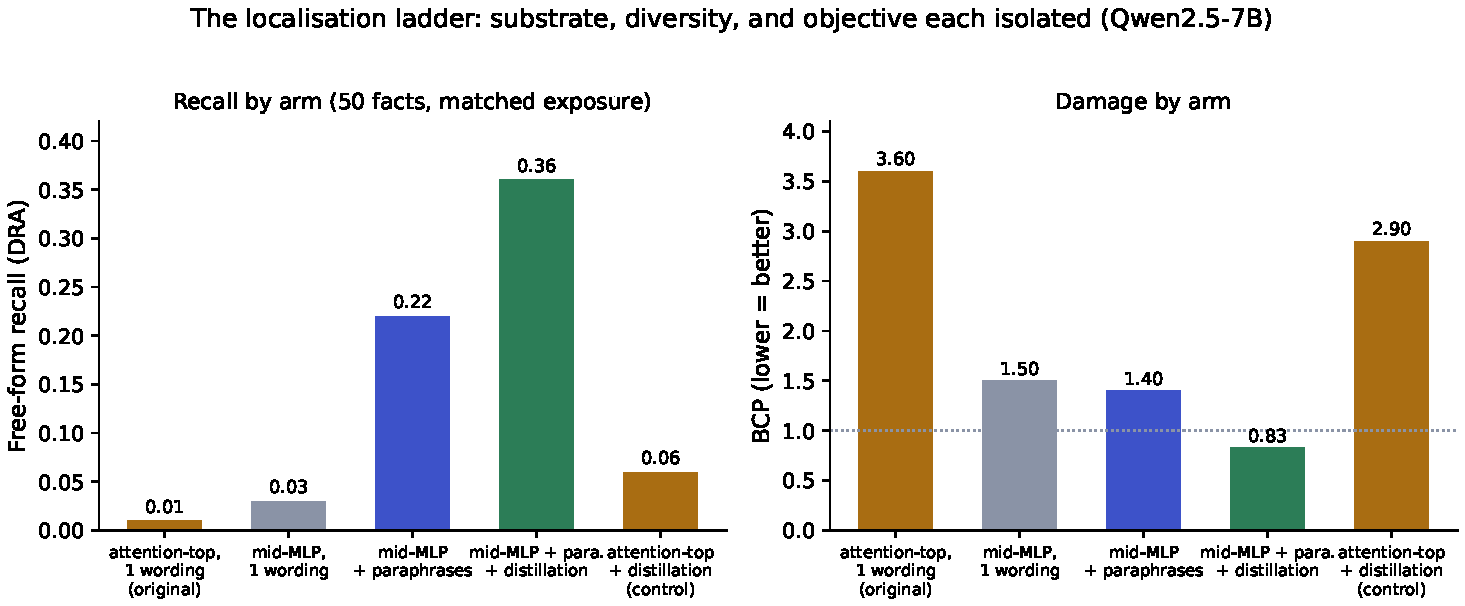
\includegraphics[width=0.98\textwidth]{figures/figure_localisation_ladder.pdf}
\caption{The localisation ladder (Qwen2.5-7B, 50 facts, matched exposure, clipping disabled; seed means---the mid-MLP single-wording arm's BCP spans $1.2$--$1.8$ across seeds and is drawn at its midpoint). Left: free-form recall by arm. Right: background damage. The same gradient budget, redirected from top-third attention to mid-stack MLPs, does less harm; paraphrase diversity and the distillation objective then convert the placement gain into recall---$60\times$ the original arm, at \emph{better}-than-baseline preservation. The placement control (rightmost) shows the objective cannot rescue the wrong substrate.}
\label{fig:ladder}
\end{figure}

\paragraph{Results:} Table~\ref{tab:ladder} and Figure~\ref{fig:ladder} report the ladder. Three findings, each consistent across both models and seeds. First, \emph{placement alone halves background damage in 8 of 8 comparisons} (Qwen BCP $3.6 \to 1.2$--$1.8$ at equal steps) and lifts recall off the floor---the same gradient budget, spent in the substrate the editing literature indicates, does less harm and more good. Second, \emph{paraphrase diversity converts memorization into extraction}: introducing paraphrases moves cloze and free-form recall in opposite directions ($0.56 \to 0.38$ cloze, $0.03 \to 0.22$ DRA), which is precisely the signature of the model ceasing to reproduce a token sequence and beginning to store a retrievable association. Third, \emph{distillation from the in-context teacher is the gentlest write}: the best arm reaches $\mathrm{DRA}=0.36$ at $\mathrm{BCP}=0.83$ on Qwen---sixty times the original floor, at \emph{better}-than-baseline preservation---while the placement control (same objective, original substrate) recovers almost none of it. On Llama the best arm is paraphrase-CE at $0.353$. The recall floor of the first movement was therefore not a structural property of frozen-backbone consolidation. It was a map error: the pipeline was writing to the wrong address, in the wrong format.

\subsection{The Third Cause: The Safety Machinery Erases the Write}
\label{sec:results_third_cause}

\paragraph{Setup:} The ladder ran with clipping disabled. Wiring the winning recipe into the \emph{full} autonomous pipeline---tagging, PRP selection, sleep engine, safety machinery, two-stage validation---tests whether it survives the system it must live in. We run the complete pipeline on 200 facts with the safety machinery at its designed setting ($\delta_{\max}=0.01$, plasticity scaling on), and identically with clip and scaling relaxed, three seeds each on Qwen2.5-7B.

\paragraph{Results:} As designed, the machinery nullifies the recipe: trained-subset DRA $0.007/0.007/0.007$, zero consolidations confirmed by the direct recall gate---indistinguishable from the original floor. Relaxed, the identical pipeline reaches trained-subset DRA $\mathbf{0.210 \pm 0.018}$ at $\mathrm{BCP}=0.90$--$0.99$, with 21--24 of $\sim$50 selected facts passing the external greedy recall gate: the first externally verified autonomous consolidations in the programme. The original consolidation failure therefore had \emph{three} stacked causes: wrong substrate (\S\ref{sec:results_localisation}), wrong surface statistics (\emph{ibid.}), and a safety clip calibrated so tightly that it erased the write after training performed it---consistent with the $\delta_{\max}$ saturation geometry identified in the diagnosis era. Each cause alone suffices to hold recall at floor, which is why no single-factor intervention in the first movement could move it.

\subsection{The Repaired Pipeline as an Autonomous System}
\label{sec:results_pipeline_v2}

The findings above fix the revised operating point (Section~\ref{sec:method_v2}): mid-MLP $W_{\mathrm{cons}}$, paraphrase replay, context distillation, moderate clipping ($\delta_{\max}=0.1$, scaling on), two-stage validation with the direct recall gate, greedy evaluation. At this operating point the full pipeline---wake-phase tagging and KV writes, PRP selection, autonomous sleep, external validation---achieves single-cycle trained-subset DRA of $0.189 \pm 0.031$ at $\mathrm{BCP}=0.882 \pm 0.027$ on Qwen2.5-7B across five seeds: recall statistically indistinguishable from the relaxed setting, at measurably \emph{better} preservation, with every seed below $\mathrm{BCP}=1.0$. On the frontier of Figure~\ref{fig:pareto}, whose best original point bought $\mathrm{DRA}=0.103$ at $\mathrm{BCP}=2.73$, this configuration sits far above the upper-left intersection that no diagnosis-era setting could reach. The two-stage gate confirms 16--23 consolidations per run externally---against the diagnosis era's $0.4 \pm 0.5$.

\subsection{The Validation Matrix: Three Families, Two Scales, Two Baselines}
\label{sec:results_matrix}

All results in this section were run under pre-registered gates (Section~\ref{sec:setup}); predictions were committed before execution.

\paragraph{Single-cycle generalisation (5 seeds per model):} Table~\ref{tab:matrix_single} reports the repaired pipeline across the four models; Figure~\ref{fig:arc} (page~\pageref{fig:arc}) plots these values against the diagnosis-era floor. Per-model recipes were fixed by a pre-registered tuning gate (best of distillation vs.\ paraphrase-CE at trained-subset DRA $\geq 0.10$, $\mathrm{BCP} \leq 1.5$, seed 0): distillation won everywhere it was tried (on Mistral, $0.750$ @ $1.31$ vs.\ $0.655$ @ $2.98$---the in-context-teacher write is also the gentler write). Every model exceeds the diagnosis-era floor by $17\times$ or more. The effect is \emph{strongest off the development model}---Mistral-7B, which the recipe had never touched, is the best result in the programme---which argues against the recipe being overfit to Qwen. The $1.5$B result ($0.105$, thin but gate-passing, only 10 of 42 selected facts surviving the recall gate versus 29 of 31 on Mistral-7B) suggests extraction capacity grows with scale. Llama-3.1-8B is the flagged exception: a pre-registered clip ladder ($\delta_{\max} \in \{0.1, 0.05, 0.03\}$) reduced damage monotonically ($4.35 \to 3.64 \to 2.14$) with recall degrading only slowly ($0.659 \to 0.593 \to 0.520$), but never reached the $1.5$ bar---Llama's damage is \emph{not clip-dominated}, and per-family learning-rate tuning is the named open item. It runs the matrix at $\delta_{\max}=0.03$ and is reported as \emph{not yet tuned}, not as solved.

\begin{table}[t]
\centering
\caption{The repaired pipeline across four models: single-cycle trained-subset DRA and BCP (5 seeds, mean $\pm$ SD). Recipes fixed by pre-registered tuning gates. Every model is $\geq 17\times$ the diagnosis-era floor of $\approx 0.006$; the strongest result is on the family the recipe never saw during development.}
\label{tab:matrix_single}
\begin{tabular}{llcc}
\toprule
Model & Recipe & Trained-subset DRA & BCP \\
\midrule
Mistral-7B   & distill, $\delta_{\max}{=}0.1$   & $\mathbf{0.750 \pm 0.033}$ & $1.205 \pm 0.058$ \\
Llama-3.1-8B & par.-CE, $\delta_{\max}{=}0.03$  & $0.512 \pm 0.048$ & $2.088 \pm 0.140$ \\
Qwen2.5-7B   & distill, $\delta_{\max}{=}0.1$   & $0.189 \pm 0.031$ & $0.882 \pm 0.027$ \\
Qwen2.5-1.5B & distill, $\delta_{\max}{=}0.1$   & $0.105 \pm 0.020$ & $1.043 \pm 0.016$ \\
\bottomrule
\end{tabular}
\end{table}

\begin{figure}[t]
\centering
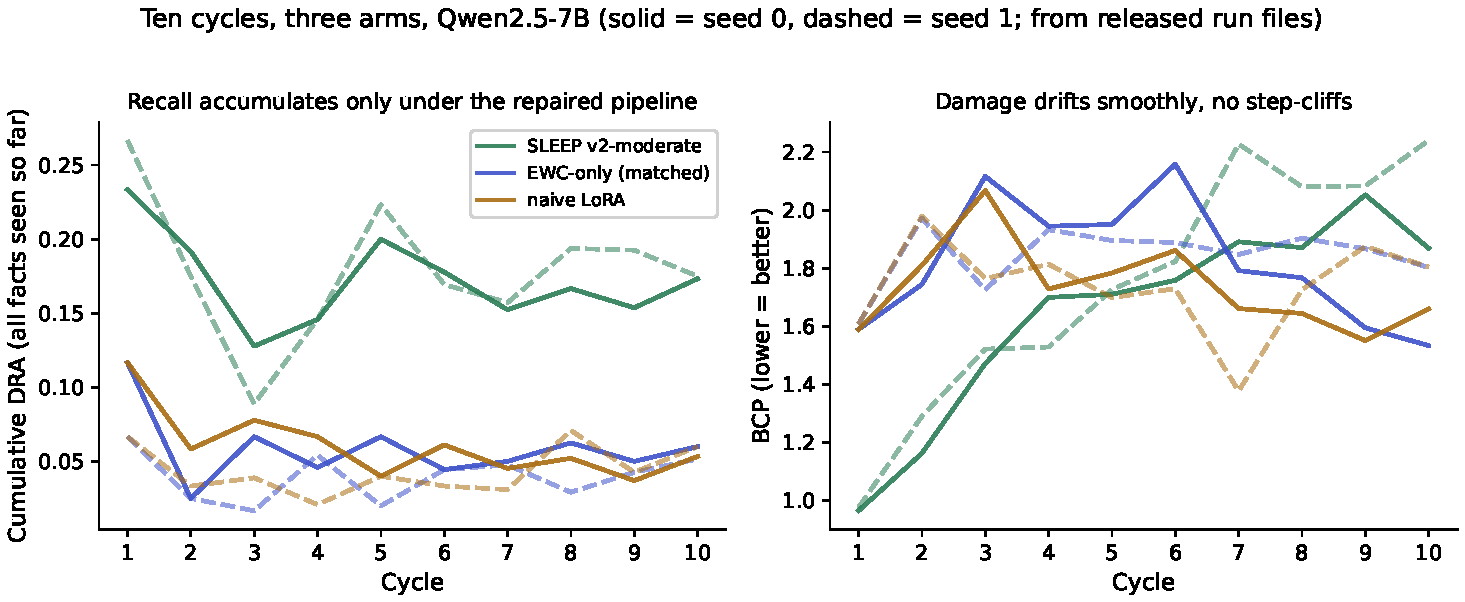
\includegraphics[width=0.98\textwidth]{figures/figure_matrix_multi_cycle.pdf}
\caption{Ten-cycle trajectories on Qwen2.5-7B, all three arms, both seeds, plotted from the released per-run result files. Left: cumulative recall over all facts seen so far---the repaired pipeline holds a $\approx 3\times$ separation above both baselines for the entire horizon, on both seeds. Right: background damage---all arms drift in the same $1.5$--$2.2$ band with no step-cliffs, in contrast to the diagnosis-era step-then-plateau signature (Figure~\ref{fig:multi_cycle}).}
\label{fig:matrix_traj}
\end{figure}

\begin{figure}[t]
\centering
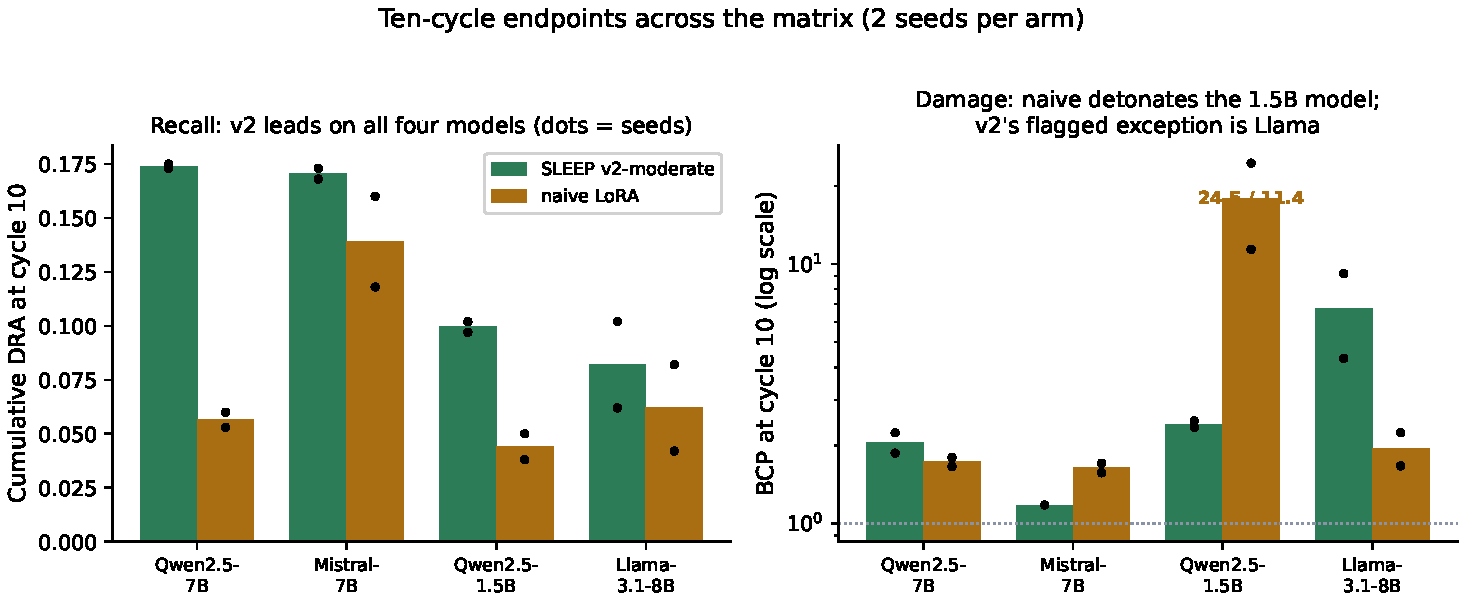
\includegraphics[width=0.98\textwidth]{figures/figure_matrix_endpoints.pdf}
\caption{Ten-cycle endpoints across the matrix (bars = seed means, dots = individual seeds). Left: the repaired pipeline leads naive LoRA on cumulative recall on all four models. Right (log scale): damage---naive LoRA detonates the 1.5B model ($\mathrm{BCP}$ $24.5$ and $11.4$, seed-random size) while the constrained arm holds $\approx 2.4$; the constrained arm's own flagged exception is Llama.}
\label{fig:matrix_endpoints}
\end{figure}

\paragraph{Ten cycles: the design-intent claim, tested (2 seeds per arm):} Table~\ref{tab:matrix_multi} and Figures~\ref{fig:matrix_traj}--\ref{fig:matrix_endpoints} repeat the ten-cycle protocol of Section~\ref{sec:multi_cycle} with the repaired pipeline (v2-moderate) against naive LoRA at the same mid-MLP adapter geometry. The pre-registered prediction---v2 exceeds naive on cumulative recall on at least two of the three newly-tested models, both seeds---was met on three of three; with Qwen2.5-7B it holds on all four models. Three regularities are seed-consistent. First, \textbf{the design-intent claim is now real}: the safety-constrained system accumulates more recall than unconstrained fine-tuning over ten cycles, $3\times$ on the anchor model. Second, \textbf{the machinery is load-bearing at small scale}: naive LoRA detonates Qwen2.5-1.5B ($\mathrm{BCP}=24.5$ and $11.4$; the blow-up size is seed-random---the plateau lottery of Section~\ref{sec:multi_cycle}, reproduced), while the constrained arm holds $\approx 2.4$ on both seeds. Third, \textbf{the constrained arm no longer exhibits the lottery}: its across-seed spread is $\approx 0.005$ DRA on every model against naive's $0.04$--$0.06$, and its damage drifts smoothly with no step-cliffs. The seed-instability finding of Section~\ref{sec:multi_cycle} thereby resolves into a property of \emph{unconstrained} arms specifically. Llama repeats its single-cycle pattern---more recall than naive on both seeds, at damage that compounds unacceptably ($\mathrm{BCP}$ $4.3/9.2$)---and keeps its flag. One qualitative signature recurs on every model: naive scores higher on \emph{current-cycle} recall while the constrained arm retains \emph{earlier} cycles better---memorization versus consolidation, now visible in the horizon dimension.

\begin{table}[t]
\centering
\caption{Ten-cycle validation: cumulative DRA at cycle 10 (seeds 0/1) with BCP. The repaired pipeline exceeds naive on cumulative recall on all four models, both seeds; at 1.5B the unconstrained arm's damage blows up seed-randomly while the constrained arm is stable.}
\label{tab:matrix_multi}
\begin{tabular}{lcc}
\toprule
Model & SLEEP v2-moderate & Naive LoRA \\
\midrule
Qwen2.5-7B   & $\mathbf{0.173/0.175}$ @ $1.87/2.24$ & $0.053/0.060$ @ $1.66/1.80$ \\
Mistral-7B   & $\mathbf{0.173/0.168}$ @ $1.18/1.18$ & $0.118/0.160$ @ $1.71/1.57$ \\
Qwen2.5-1.5B & $\mathbf{0.097/0.102}$ @ $2.35/2.49$ & $0.038/0.050$ @ $\mathbf{24.5/11.4}$ \\
Llama-3.1-8B & $0.102/0.062$ @ $4.33/9.20$ & $0.082/0.042$ @ $2.24/1.67$ \\
\bottomrule
\end{tabular}
\end{table}

\paragraph{The baseline that matters: EWC-only (matched arms):} The diagnosis era left an uncomfortable finding: EWC alone looked competitive with the full pipeline. The matrix settles it with the matched-arm comparison of Section~\ref{sec:setup} on the two headline families, ten cycles, two seeds (Table~\ref{tab:matrix_ewc}). The pre-registered prediction held exactly: the penalty gives EWC-only the best damage numbers, but its recall sits at naive's level---\textbf{regularization prevents forgetting; it does not create extraction}. The repaired pipeline delivers $3\times$ the cumulative recall of both baselines on Qwen2.5-7B at comparable damage, passing the pre-registered headline gate. On Llama, EWC-only is competitive with the not-yet-tuned v2 ($0.075/0.072$ at far better BCP)---reported plainly: the Llama column is not a v2 win.

\begin{table}[t]
\centering
\caption{The EWC showdown: cumulative DRA at cycle 10 (seeds 0/1) with BCP, matched-arm EWC. On the anchor model the repaired pipeline triples both baselines' recall at comparable damage; EWC's penalty preserves but does not create recall.}
\label{tab:matrix_ewc}
\begin{tabular}{lccc}
\toprule
Model & SLEEP v2-moderate & EWC-only & Naive LoRA \\
\midrule
Qwen2.5-7B   & $\mathbf{0.173/0.175}$ @ $1.87/2.24$ & $0.060/0.052$ @ $1.53/1.80$ & $0.053/0.060$ @ $1.66/1.80$ \\
Llama-3.1-8B & $0.102/0.062$ @ $4.33/9.20$ & $0.075/0.072$ @ $2.32/1.79$ & $0.082/0.042$ @ $2.24/1.67$ \\
\bottomrule
\end{tabular}
\end{table}

\paragraph{Residual gaps, named:} Three limitations survive the matrix and are carried explicitly into future work. Background damage leaks $\approx +0.12$ BCP per cycle in every arm---no configuration holds $\mathrm{BCP} < 1.05$ over ten cycles. Early-cycle batches fade in cumulative recall because the engine rehearses only the current batch; interleaved rehearsal of prior consolidations---the mechanism biological sleep actually implements---is the clearest next component. And Llama-3.1-8B requires per-family optimisation before its recall gains are usable.
